\PassOptionsToPackage{top=3cm,left=3cm,right=3cm,bottom=3cm}{geometry}
\documentclass[fleqn,11pt]{wlscirep}

\usepackage{import}
\usepackage{main}

\renewcommand{\paragraph}[1]{\vspace{0.3cm}\noindent\underline{\emph{#1}}\hfill\noindent}

% word count
% \newcommand{\maincount}[1]{%
%   \immediate\write18{texcount -1 -sum=1 -merge -q -nobib #1.tex > #1-words.sum}%
%   \input{#1-words.sum}%
% }

% \newcommand{\abstractcount}[1]{%
%   \immediate\write18{texcount -template="{abst}" #1.tex > #1-words.sum}%
%   \input{#1-words.sum}%
% }

\begin{document}

\doublespacing

\title{\bfseries\LARGE\singlespacing{Spatiotemporal modeling of \emph{Mycobacterium tuberculosis} transmission risk in a South African primary care clinic using environmental, clinical, and patient movement data}}
% author list
\author[1$\ddag$]{Nicolas Banholzer}
\author[2]{Keren Middelkoop}
\author[2]{Juane Leukes}
\author[1]{Kathrin Zürcher}
\author[1]{Matthias Egger}
\author[2]{Robin Wood}
\author[1*]{Lukas Fenner}

\affil[1]{Institute of Social and Preventive Medicine, University of Bern, Bern, Switzerland}
\affil[2]{Desmond Tutu HIV Centre, Department of Medicine, University of Cape Town, Cape Town, South Africa}

\affil[*]{Corresponding author: lukas.fenner@unibe.ch }

\vspace{1em}

% \begin{information}\normalfont
% \noindent\textbf{Running head}: SARS-COV-2 transmission in schools and effect of air cleaners

% %\noindent\textbf{Subject categorization}: 6.20  Indoor Air; 10.11 Pediatrics: Respiratory Infections

% \noindent\textbf{Word count}: \maincount{manuscript}words, abstract \abstractcount{manuscript}words (max. 500), title 157 chars (max. 200)

% %\noindent\textbf{Inserts:} 2 tables, 6 figures, 44 references

% \noindent\textbf{S1 Appendix:} Includes supplementary text, tables and figures.

% \vspace{1em}

% \noindent\textbf{Funding}

% \noindent This study is funded by the Multidisciplinary Center for Infectious Diseases, University of Bern, Bern, Switzerland. NB, LF, and ME are supported by the National Institute of Allergy and Infectious Diseases (NIAID) through cooperative agreement 5U01-AI069924-05. ME is supported by special project funding from the Swiss National Science Foundation (grant 32FP30-189498). \medskip

% \noindent\textbf{Contributions}

% \noindent Conception and design: NB, LF. Epidemiological and environmental data collection: NB, PJ, TS, LF. Laboratory data collection: PB, LFu. Additional data collection: TH. Statistical analysis: NB, KZ. Genomic analysis: LB, LFu. Paper draft: NB, LF, ME. All authors reviewed and approved the final version of the manuscript.

% \par
% \end{information}

%TC:newcounter abst Words in abstract
%TC:envir abstract [] abst
\begin{abstract}\normalfont
\noindent\textbf{Background:} Tuberculosis (TB) caused by \emph{Mycobacterium tuberculosis (Mtb)} was the leading cause of death from any single infectious disease before the COVID-19 pandemic. TB is strictly airborne and thus the transmission risk is higher in crowded indoor settings, especially healthcare facilities. Existing approaches to model the risk of airborne transmission typically assume that the airspace is well mixed, thereby ignoring that closer proximity to infectious individuals may increase the risk of transmission.

\noindent\textbf{Methods:} We developed a spatiotemporal extension of the Wells-Riley model to estimate the risk of \emph{Mtb} transmission using environmental (CO$_2$ levels), clinical data (patient visits and TB disease status), and patient movement data (anonymous patient tracking from video sensors). The data were collected for five days in October/November 2021 in a primary care clinic in Cape Town, South Africa. We matched patient movements with clinical records to identify the spatiotemporal location of TB infectious patients. Based on that, we modeled the spatiotemporal concentration of infectious doses and estimated the patient-specific risk of infection using Monte Carlo simulation.

\noindent\textbf{Results:} Clinical records registered 894 patients visiting the clinic, four of which were diagnosed with TB. Patient movement data suggested 1,438 people visiting the clinic (median stay 25\,min, interquartile range [IQR] 13\,min$-$46\,min). CO$_2$ levels were mostly below 600\,ppm, suggesting that the clinic was very well ventilated. The modeled mean risk of infection was 7\% (95\%-credible interval [CrI] 0.5\%$-$31.1\%) and the risk was significantly associated with the number of close-contact encounters, time spent in the clinic, and the air change rate. Without infection control measures that were implemented during the COVID-19 pandemic, the modeled risk of infection would have been 7.8\% (95\%-CrI 0.4\%$-$41.3\%) without mask wearing and 8.4\%-CrI 0.6\%$-$41.4\%) with lower ventilation.

\noindent\textbf{Conclusions:} Risk of \emph{Mtb} transmission in primary care clinic in South Africa is considerable, especially for attendees with many close-contact interactions. Infection control measures probably mitigated the risk of \emph{Mtb} transmission. Our spatiotemporal model could be used in future work to assess the impact of measures preventing prolonged close contact with potentially infectious patients. 

\par
\end{abstract}

%TC:ignore

\flushbottom
\maketitle
\setcounter{page}{1}
\thispagestyle{fancy}

\vspace{2em}

%\noindent\textbf{Word count:} \abstractcount{manuscript}words (max. 500)

\vspace{0.5em}

\noindent\textbf{Keywords:} Mycobacterium tuberculosis, patient movements, Wells-Riley model
% maximum of 3-5 keywords
\newpage

\sloppy
\raggedbottom
%TC:endignore

\newpage

%TC:break main
\section{Introduction} 

% TB and the route of transmission
Tuberculosis (TB) is one of the leading causes of death worldwide, especially in the South-East Asian and the African region, and progress made in TB prevention and control before the COVID-19 pandemic has stalled or reversed\cite{WHO2022TBReport}. \emph{Mycobacterium tuberculosis} (\emph{Mtb}), the causative agent of TB, transmits via respiratory particles in the exhaled air of infectious persons\cite{Rieder1999,Patterson2021Tuberculosis}. \emph{Mtb} is carried primarily in smaller particles in the size range of $2\mu$m to $5\mu$m\cite{Fennelly2020Lancet}, which can survive in the air for multiple hours\cite{Loudon1969AMRRD}. Airborne survival is greater in crowded, poorly ventilated indoor settings\cite{Rieder1999,CPS2013Book,Nardell1991ARRD,Wang2021Science,Morawska2021} and healthcare facilities present a particular high-risk setting because both people that are more infectious and susceptible also more frequently visit the clinic\cite{McCreesh2020IJTLD}. A study in South Africa estimated that 4\% to 14\% of TB cases in adults originate from primary care clinics\cite{McCreesh2022BMJGlobalHealth}.

% the Wells-Riley model and its limitations
The Wells-Riley model\cite{Riley1978AJE} is frequently used to estimate the risk of airborne transmission in a variety of indoor settings\cite{Andrews2014JID,Taylor2016IJTLD,Hella2017JInfect,Zemouri2020JDR}, including primary care clinics\cite{Zurcher2022JID,McCreesh2021BMJGlobalHealth}. The model assumes estimates the risk of infection based on the number of infectious individuals in space, the generation rate of infectious quanta (doses of pathogen-carrying particles), the breathing rate per person, and the outdoor air supply rate. The Wells-Riley, and variations thereof\cite{Rudnick2003IndoorAir}, assume a well-mixed airspace, which means that the quanta concentration is the same everywhere in the room. However, the quanta concentration is typically higher near the infectious source\cite{Wang2021Science,Vuorinen2020SafSci,Chen2020BuildEnv}, and previous studies showed that the risk of TB infection is associated with proximity to these individuals\cite{Ko2004RiskAnal,Kenyon1996NEJM}.

% what this study adds
We build on the Wells-Riley model and develop a spatiotemporal extension to model the concentration of infectious quanta spatially and over time. We combine clinical and video sensor data to identify the spatiotemporal location of TB infectious and susceptible patients visiting a primary care clinic in South Africa during five days in October/November 2021. Furthermore, we measure indoor CO$_2$ levels to model the spatial diffusion and removal of infectious quanta over time. Using Monte Carlo simulation, our model allows us to estimate the risk of infection individually for each clinical attendee. Furthermore, we estimated the impact of infection control measures which were in place during the COVID-19 pandemic using hypothetical scenarios.

\newpage

\section{Methods}

\subsection{Study design}

We build on the design of a pilot study in 2019\cite{Zurcher2022JID}, which was described in detail in a study protocol \cite{Zurcher2020BMJ}. We collected environmental data (indoor CO$_2$ levels), clinical data (TB status), and video sensor data (patient movements) for five days during the COVID-19 pandemic in October/November 2021 (October 13, 15, 25, and November 4, 5) at a primary care clinic in Cape Town, South Africa. 

\subsection{Study setting}

The primary care clinic offers both TB and HIV services and other basic clinical services, Monday to Friday, from 8\,am to 4\,pm. The clinic is situated within a large settlement of formal and semiformal housing where both TB and HIV are highly prevalent\cite{Wood2007AMJRCCD,Middelkoop2011JAIDS}. We defined three areas within the clinic (\Cref{fig:floor-plan}): the waiting room (10.55m $\times$ 5.50m $\times$ 3.00m), corridor (12.45m $\times$ 2.20m $\times$ 2.50m), and TB room (4.75m $\times$ 3.50m $\times$ 3.00m). The TB room was primarily used for diagnosed TB patients and suspected patients with respiratory symptoms.

\begin{figure}[!htpb]
    \centering
    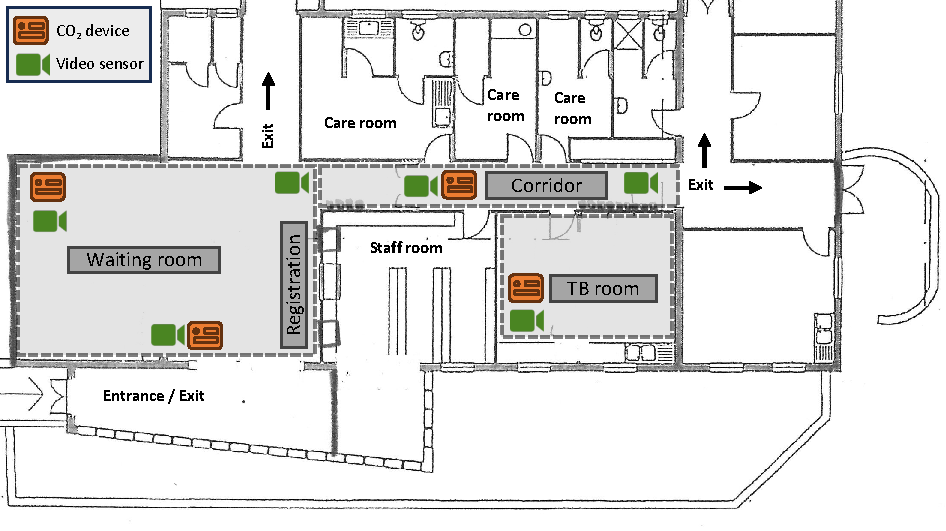
\includegraphics{doc/clinic-schematic-annotated-view.pdf}
    \caption{\textbf{Schematic view of the clinic}. Patients typically enter the clinic through the entrance on the bottom left, register at the reception, then wait in the waiting room or along the corridor until they see a doctor in one of the care rooms or the TB room, and finally exit the clinic through one of the exits in the waiting room or at the end of the corridor. Colored icons show the placement of the video sensors to track patient movements and the devices monitoring CO$_2$ levels.}
    \label{fig:floor-plan}
\end{figure}


\subsection{Data}

\subsubsection{Environmental data}

Four devices monitored indoor CO$_2$ levels (Digital CO$_2$ Monitor Carbon Dioxide Meter XE-2000, XEAST, Guangdong, China) in the waiting room, corridor, and TB room (\Cref{fig:floor-plan}). CO$_2$ levels were recorded in parts per million (ppm) at 1min intervals. Missing values were linearly imputed. On October~13, the corridor's CO$_2$ levels were missing and imputed with the waiting room's CO$_2$ levels because their CO$_2$ measurements were similar on the other study days.    

\subsubsection{Clinical data}

We extracted clinical data from the electronic patient registry for all patients who visited the clinic during the study period. These data included the date and time of arrival, TB diagnostic results, and date of TB treatment start. We defined infectious patients as individuals testing bacteriologically positive for TB during the study or being on TB treatment for less than four weeks. Patients who had been treated for more than four weeks or recently completed a treatment were neither considered infectious nor susceptible. We also defined suspected TB patients as individuals who were tested for TB following symptom screening, but who were subsequently not diagnosed with TB. 

\subsubsection{Tracking data}

We used an anonymous personal tracking system (Xovis, Zollikofen, Switzerland) to monitor the movements of people (clinical staff, patients, and other visitors) throughout the clinic at 1s intervals (\Cref{fig:floor-plan}). The resulting timestamped movement data consisted of a person’s height, their position recorded as x-y coordinates, and a unique ID for each person's track while in the clinic. \supp Figure~\zref{fig:tracking-examples} shows a few sample tracks from our study. Note that individuals could contribute multiple tracks if they moved out of the sensor's range or were briefly not recognized as a person. To remedy these issues, we created an R Shiny tool to manually link interrupted tracks back together (\supp Text~\zref{sec:setting-and-data}). Furthermore, we labeled tracks to identify movements from clinical staff.  

\subsection{The Wells-Riley equation}

Our spatiotemporal model builds upon the Wells-Riley equation\cite{Riley1978AJE}, which estimates the risk (probability) of infection $P$ as
\begin{align}
    P = \frac{D}{S} = 1 - \exp\left(\frac{Ipqt}{Q}\right),
\end{align}
where $D$ is the number of diseases cases, $S$ is the number of susceptible cases, $I$ is the number of infectious people in the indoor space, $p$ is the breathing rate (m$^3$ s$^{-1}$), $q$ is the quantum (infectious dose) generation rate (quanta s$^{-1}$), $t$ is the exposure time (s), and $Q$ is the ventilation rate (m$^3$ s$^{-1}$). The probability of infection is estimated with a Poisson relation, considering the stochastic behavior of airborne infection, where one quantum corresponds to a 67\% risk of infection. The main assumption of the Wells-Riley model is a well-mixed airspace, which means that the quanta concentration $N = Iq/Q$ (quanta m$^{-3}$) is the same everywhere in the room. Our aim is to relax this assumption by using patient movement data to identify the location of infectious patients and consider spatial variation in the quanta concentration. 

\subsection{Spatiotemporal modeling approach}

A detailed description of the Wells-Riley model and our spatiotemporal extension is provided in \supp Text~\zref{sec:spattemp-model}. In the following, we describe the main components of our modeling approach, which are summarized in \Cref{fig:modeling-flow}.

\begin{figure}[!htpb]
    \centering
    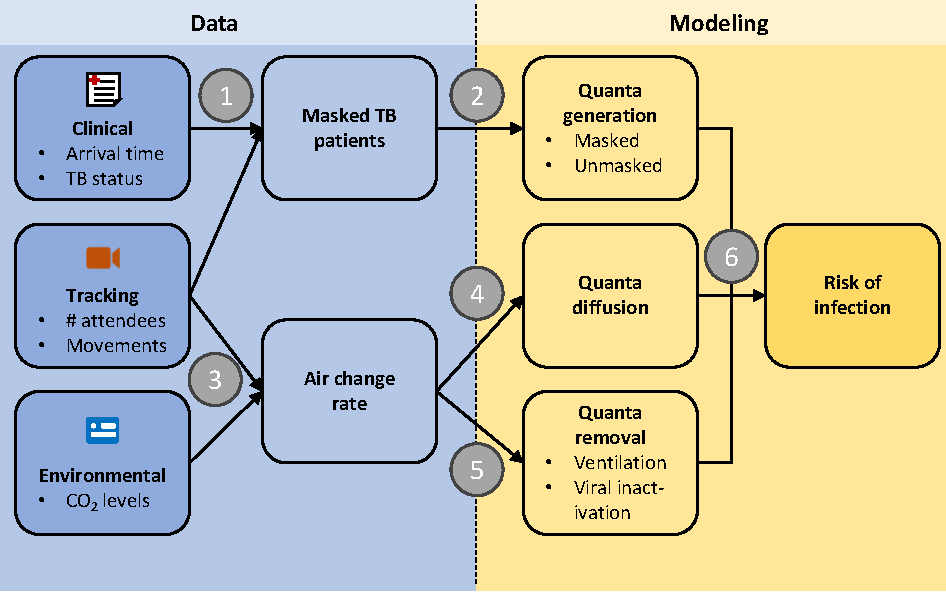
\includegraphics{doc/paper/flow-chart.pdf}
    \caption{\textbf{Visual summary of the spatiotemporal modeling approach}. (1)~Clinical and tracking data is combined to identify the spatiotemporal location of diagnosed (infectious) TB patients. (2)~Both diagnosed and randomly sampled undiagnosed  patients among visitors generate infectious quanta. (3)~Tracking and environmental data is combined to estimate the air change rate. (4)~The air change rate is related to the speed with which quanta diffuses in the indoor space. (5)~The air change rate also determines quanta removal through outdoor air exchange, in addition to inactivation of \emph{Mtb} in airborne particles. (6)~Quanta generation, diffusion, and removal determine the spatiotemporal quanta concentration, based on which the personal risk of infection is computed.}
    \label{fig:modeling-flow}
\end{figure}

\subsubsection*{Quanta generation}

(1)~We matched clinical and patient movement data to identify the spatiotemporal location of infectious TB patients inside the clinic. We recorded the timestamp when the patient movement was in the registration area and matched this with the registration time in the clinical records. We excluded patient movements of less than five minutes and with less than five seconds in the registration area from the matching. Data were matched if there was a patient movement in the registration area followed by a entry in the clinical database, considering a maximum delay of 15 minutes. All diagnosed TB patients could be matched with patient movements this way. (2)~In addition to diagnosed TB patients, we also consider a number of undiagnosed patients. Prior studies suggest that the number of undiagnosed TB patients is proportional to the number of diagnosed TB patients \cite{Berhanu2023CID}. Therefore, we model the number of undiagnosed TB patients with a multinomial distribution based on the counts of the daily number of diagnosed patients in the clinical data in October/November 2021 (\supp~Figure~\zref{fig:count-tb-patients}): 6 (12\%) days with zero, 12 (41\%) with one, 8 (28\%) with two, 2 (7\%) with three, and 1 (3\%) with four visiting TB patients. Undiagnosed patients were randomly sampled among all visitors with the same probability. Clinical staff were not considered infectious and excluded from the sampling. We assumed that diagnosed and undiagnosed TB patients generated quantum at the same rate $q$, which was modeled using a lognormal prior distribution and considering two different activity levels (\supp~Figure~\zref{fig:quanta-distribution}): median 1.08\,quanta h$^{-1}$ (95\%-credible interval [CrI] 0.003\,quanta h$^{-1}$\,$-$\,386\,quanta h$^{-1}$) while sitting and 2.81\,quanta h$^{-1}$ (95\%-CrI 0.008\,quanta h$^{-1}$\,$-$\,987\,quanta h$^{-1}$) while walking\cite{Mikszewski2021GF,Buonanno2020EI,Banholzer2024PGPH}. Since mask wearing was mandatory for all clinical staff and visitors during the study, we assumed a mean reduction in $q$ by 75\% (95\%-CrI 56\%\,$-$\,86\%)\cite{Dharmadhikari2012AJRCCM,McCreesh2021BMJGlobalHealth}.

\subsubsection*{Quanta diffusion}

(3)~We calculated room occupancy from the video sensor data and combined it with the CO$_2$ measurements to estimate air change rates by daytime using a transient mass balance model\cite{Batterman2017IJERPH}. (4)~The air change rate was related to the diffusion of quanta using, as an approximation, the empirical relationship between the eddy diffusion coefficient and the air change rate in CO$_2$ particles\cite{Cheng2011EnvSciTech,Foat2020BE}. Since airflow was not monitored in our study, we assume that the quanta diffuse radially from where they were generated (\supp~Figure~\zref{fig:toy-example}). 

\subsubsection*{Quanta removal}

(5)~Quanta removal occurs through replacement of contaminated indoor air with fresh outdoor air, inactivation of bacteria in airborne particles, and gravitational settling. The removal rate is thus the sum of the air change rate, the inactivation rate of \emph{Mtb}, and the gravitational settling rate. The bacterial inactivation rate was modeled using a lognormal prior distribution (\supp~Figure~\zref{}) with a median of 1\,quanta h$^{-1}$ (0.1\,quanta h$^{-1}$\,$-$\,7.1\,quanta h$^{-1}$)\cite{Loudon1969AMRRD,Lever2000LettersAppliedMicrobio,Gannon2007ResVetSci,Klein2014IJMyco}. We set the gravitational settling rate to zero, thereby ignoring sedimentation because the particles carrying \emph{Mtb}, which are in the size range of $2\mu$m to $5\mu$m\cite{Fennelly2020Lancet}, are airborne immediately or within seconds\cite{Vuorinen2020SafSci}.

\subsubsection*{Risk of infection}

(6)~Based on the quanta generation, diffusion, and removal process, the quanta concentration $N$ (quanta\,m$^{-3}$) at time $t$ was computed as 
\begin{align}\label{eq:spattemp-N}
    \underbrace{N_{t}}_{\text{new concn.}} = \underbrace{\left(D \Delta (\underbrace{N_{t-1}}_{\text{prev. concn.}} + \underbrace{I_t \cdot q}_{\text{generation}})\right)}_{\text{diffusion}} \cdot \underbrace{\exp\left(-(AER_t + \lambda)\right)}_{\text{removal}} ~.
\end{align}
where $D$ is the diffusion constant (m$^2$ s$^{-1}$), $\Delta$ is the Laplace operator (second-order differential operator), $I_t$ is the number of infectious individuals in space, $q$ is the quantum generation rate (quanta s$^{-1}$), $AER$ is the air change rate (quanta\,s$^{-1}$), and $\lambda$ is bacterial inactivation rate (quanta s$^{-1}$). The patient-specific risk of infection depends on the cumulative exposure to infectious quanta and was computed using the Wells-Riley equation as
\begin{align}
    P = 1-\exp\left(-\sum_c \sum_t N_{c,t} \cdot \mathbb{I}_{c,t} \cdot p_a\right),
\end{align}
where $N_{s,t}$ is the quanta concentration in cell space $c$ at time $t$, $\mathbb{I}_{c,t}$ is indicates whether the attendee was in $c$ at time $t$, and $p_a$ (m$^3$ s$^{-1}$) is the breathing rate for activity level $a$. We distinguished between walking ($p_\mathrm{walk}$ = 1.33\,m$^3$ h$^{-1}$) and sitting activities ($p_\mathrm{sit}$ = 0.51\,m$^3$ h$^{-1}$)\cite{Adams1993}, based on whether the distance between two patient tracks was more or less than 0.25m.

\subsection{Monte Carlo simulation}

The model setup and simulation approach is described in detail in Text~\zref{sec:estimation}, including a comprehensive review of our modeling assumptions and prior distributions. To summarize, we simulated the spatiotemporal quanta concentration separately for the waiting room, corridor, and TB room of the clinic. Each room was rasterized into a grid of cubic cells with a squared area of 0.25m$^2$. The quanta concentration was modeled during clinic hours from 8am to 4pm and updated every second. We used a Monte-Carlo simulation approach to consider uncertainty in key modeling parameters. In each simulation, we sampled uncertain modeling parameters from their prior distributions and, based on that, computed the spatiotemporal quanta concentration and the risk of infection per clinical attendee. 

\subsection{Hypothetical scenarios}

Our study was set during the COVID-19 pandemic when infection control measures were in place. To model their effectiveness, we considered two hypothetical scenarios: 1)~no mask wearing, \ie assuming no reduction in the quantum generation rate; and 2)~lower ventilation, \ie a fixed air change rate of 16 air changes per hour, corresponding to the average in our pilot study of 2019 before the pandemic\cite{Zurcher2022JID}. Furthermore, we examined the impact of different assumptions regarding the number infectious patients in space: 1)~instead of undiagnosed TB patients, we considered suspected TB patients as infectious; 2)~random sampling of infectious patients among all visitors in proportion to the prevalence of TB in the South African population\cite{Moyo2022LancetID}. Except for the scenario-specific modifications, all other modeling assumptions and parameters were the same in each Monte Carlo simulation, ensuring comparability of the results. 

\subsection{Statistical analysis}

Clinical (diagnosed and suspected TB patients), environmental (time-varying CO$_2$ levels and air change rates) and patient movement data (spatiotemporal number of tracks, visit time, and close-contact encounters) were assessed descriptively and summarized with the median and interquartile range (IQR). Spatiotemporal quanta concentration and risk of infection per clinical attendee were estimated based on 5,000 Monte Carlo simulations. The average quanta concentration was computed by daytime (morning: 8am to 12am, afternoon: 12am to 4pm) and the risk of infection was summarized with the mean/median and 95\%-credible interval (CrI). A Bayesian Beta regression model was used to estimate the odds ratio (OR) of the modeled risk of TB infection in association with the air change rate, visit time, and close-contact encounters. All analyses were performed in R software (version 4.3.1) and the Bayesian regression model was estimated in the probabilistic programming language Stan (version 2.26.1).


\subsection{Ethics statement}

The University of Cape Town Faculty of Health Sciences Human Research Ethics Committee (HREC/REF: 228/2019), the City of Cape Town (Project ID: 8139), South Africa, and the Ethics Committee of the Canton of Bern (KEK/REF: 2019-02131), Switzerland, approved the study.

\newpage

\section{Results}

During the five study days, 894 patients have been registered in the clinical database, of which four patients were diagnosed with TB and 16 patients were suspected of TB following symptom screening (\supp~Figure~\zref{fig:diagnosed-tb-patients}). Overall, 1,563 unique movements were detected in the clinic after processing the video sensor data, of which 125 were labeled as being from healthcare workers, identifying 1,438 patients or other visitors. Most movements were detected in the waiting room (\Cref{fig:input-data-descriptives}a) and during the morning (\Cref{fig:input-data-descriptives}b). Patients spent around half an hour in the clinic (median 25\,min, IQR 13\,min$-$46\,min), most of it in the waiting room (\Cref{fig:input-data-descriptives}c). Close-contact encounters (distance <1\,m and duration >1\,min) were frequent (median 5, IQR 2$-$9), and several patients had more than ten close contacts during their visit (\Cref{fig:input-data-descriptives}d). The majority of patients was in close contact with at least one other person for more than half the time of their visit (median 68\%, IQR 41\%$-$87\%, \Cref{fig:input-data-descriptives}e). The CO$_2$ levels inside the clinic were low (median 431\,ppm, IQR 406\,ppm$-$458\,ppm (\Cref{fig:input-data-descriptives}f) and the corresponding air change rates were high (\Cref{fig:input-data-descriptives}g), especially the densely occupied waiting room (median 29\,h$^{-1}$), IQR 9\,h$^{-1}$$-$36\,h$^{-1}$). 


\begin{figure}
    \centering
     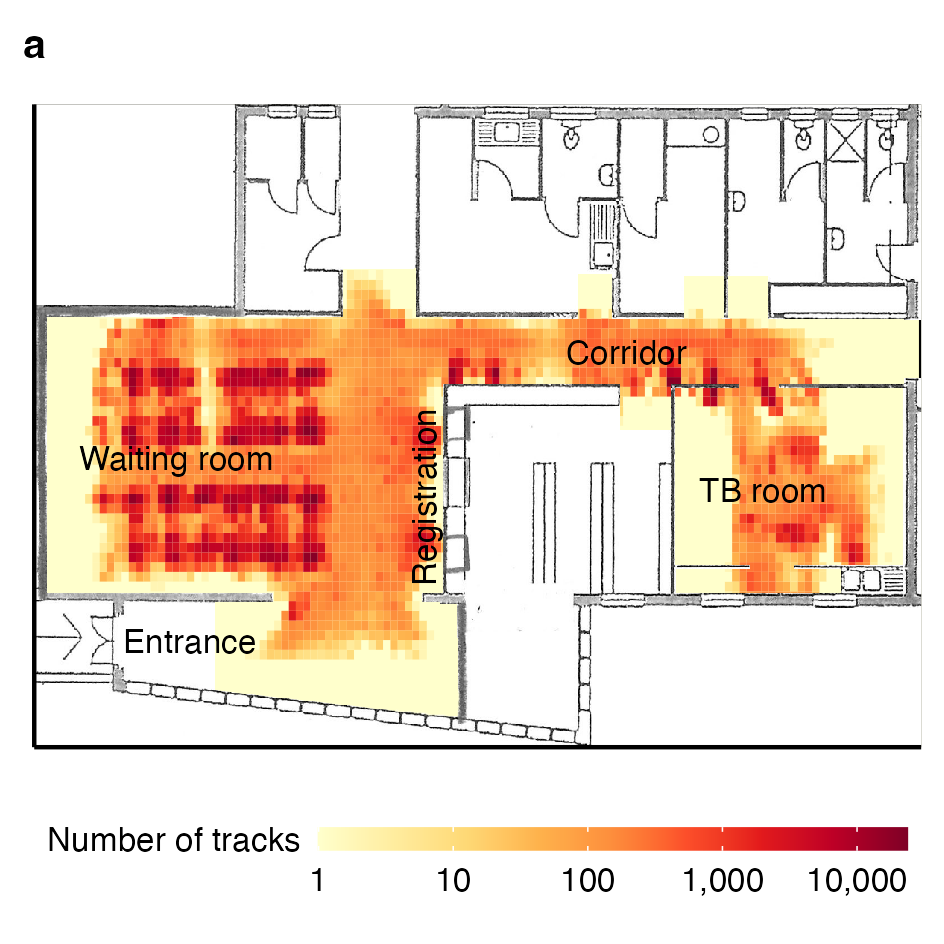
\includegraphics{results/data/no-people-spatial.png}
    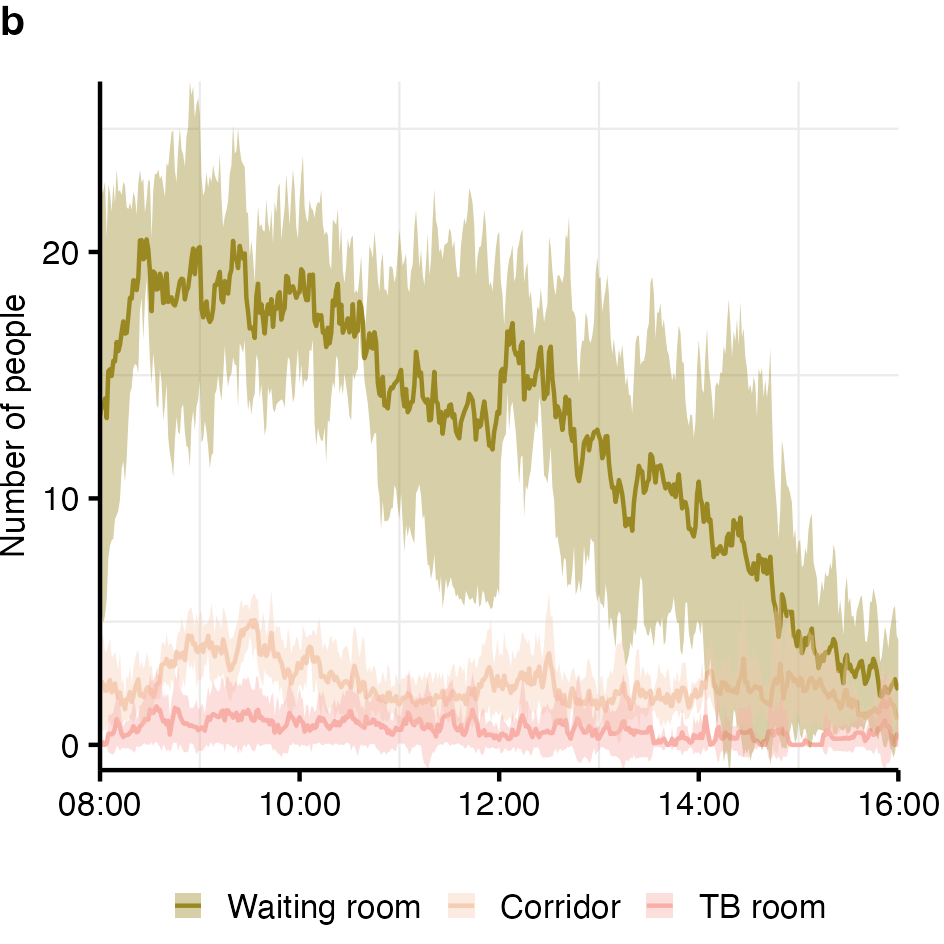
\includegraphics{results/data/no-people-over-time.png}
    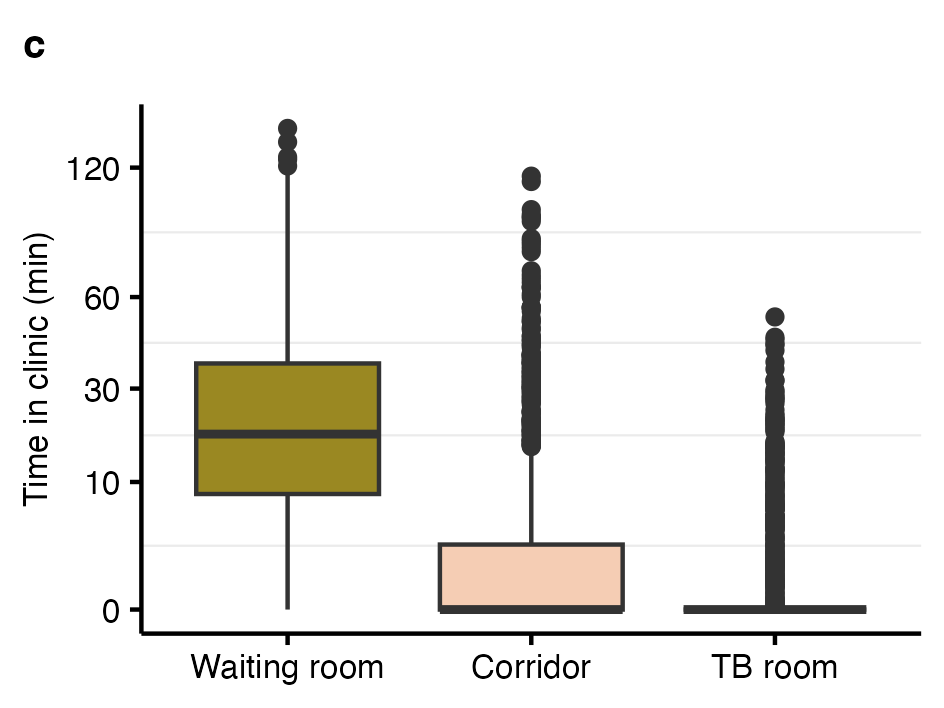
\includegraphics{results/data/time-in-clinic.png}
    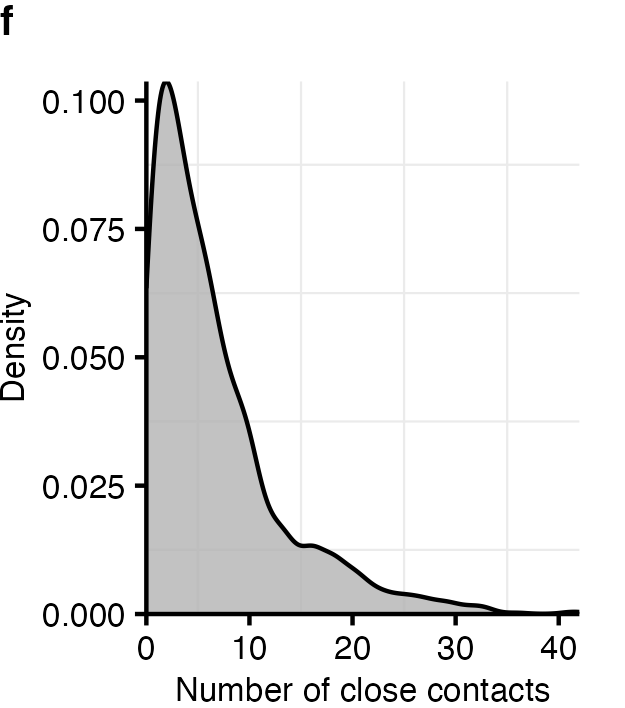
\includegraphics{results/data/number-close-contacts.png}
    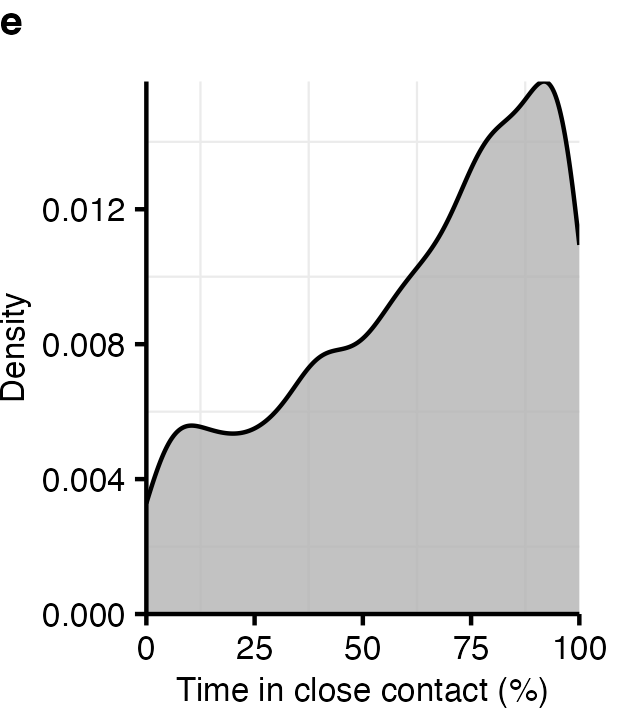
\includegraphics{results/data/time-close-contacts.png}
    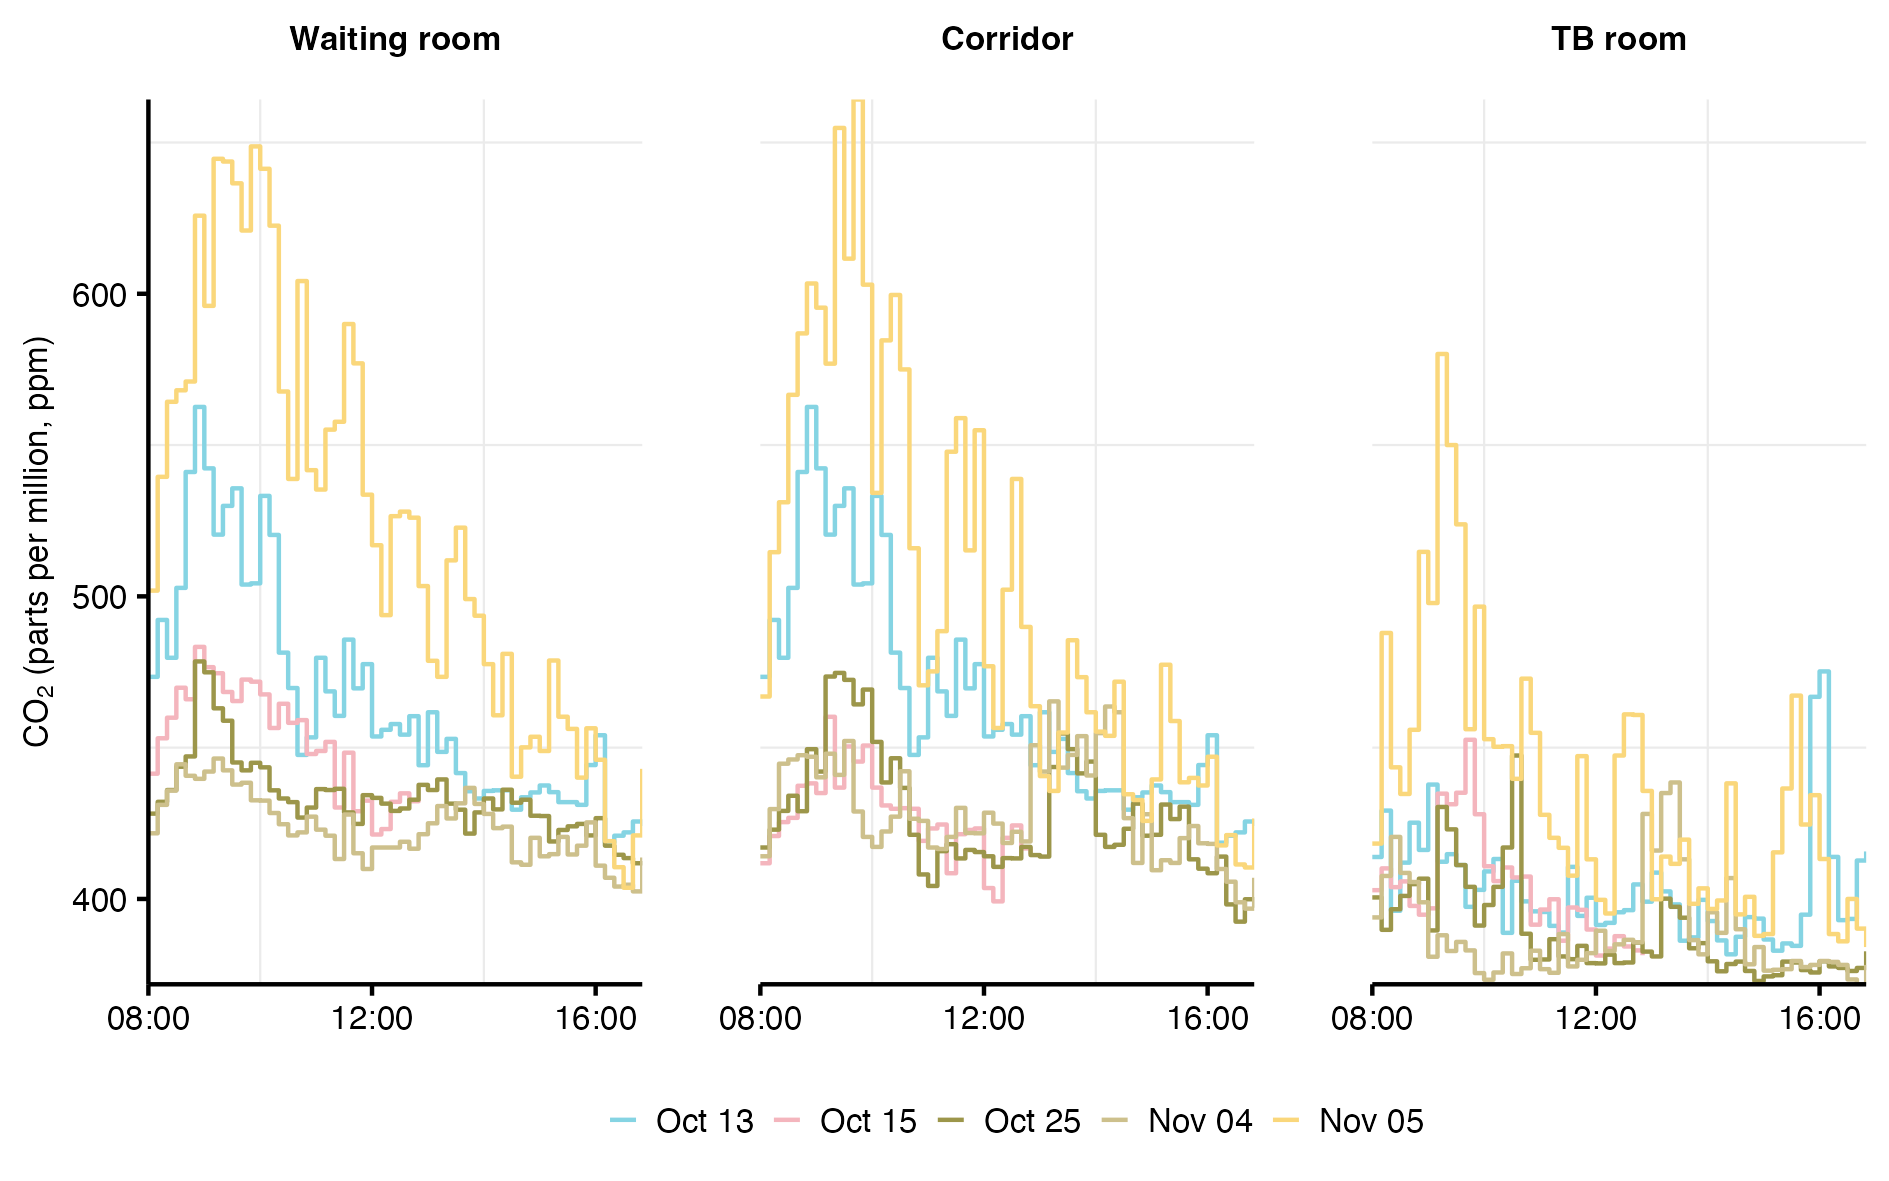
\includegraphics{results/data/co2-levels-over-time.png}
    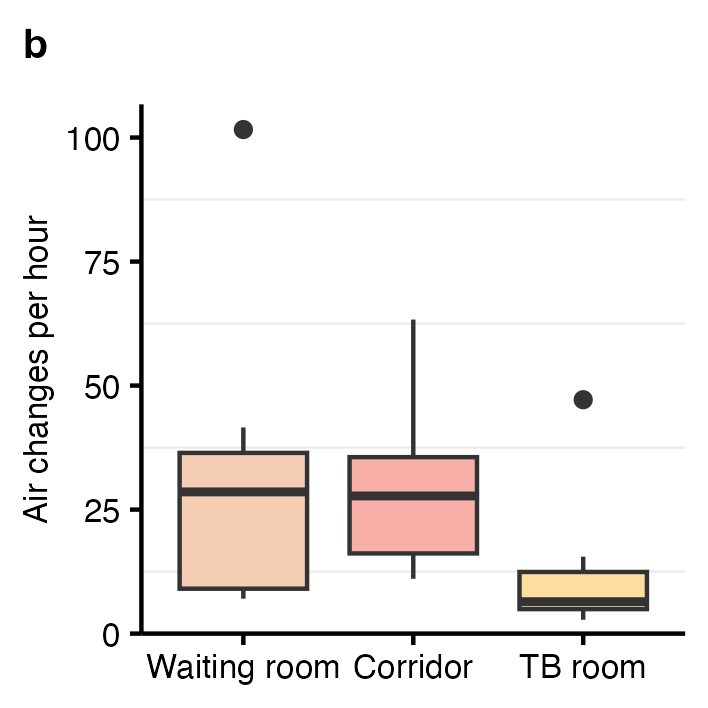
\includegraphics{results/data/air-changes-per-hour.png}
    \caption{\textbf{Environmental conditions and patient movement characteristics.} \textbf{(a)}~CO$_2$ levels per room of the clinic over time per day. \textbf{(b)}~Air change rates per room of the clinic. \textbf{(c)}~Total number of tracks recorded per unit space in the clinic over the study period. \textbf{(d)}~Number of people in the clinic over time per day. \textbf{(e)}~Time spent in the clinic per clinical attendee. \textbf{(f)}~Density distribution of the number of close contacts per clinical attendee during their visit. \textbf{(g)}~Density distribution of the time spent in close contact per clinical attendee during their visit.}
    \label{fig:input-data-descriptives}
\end{figure}

As an illustrative example of our spatiotemporal model, the animation in \supp File 2 shows the spatiotemporally varying quanta concentration as an infectious patient enters the clinic in the morning of October 25 and moves through the waiting room. The quanta concentration is higher near the infectious patient, therefore indicating his position and movement. It can further be seen that the quanta diffuses fairly quickly due to its relation with the air change rate, which was very high because all doors and windows were typically open in the clinic. \Cref{fig:main-modeling-results} shows the results from our main spatiotemporal modeling analysis across study days and simulations. The mean quanta concentration was higher in the morning than in the afternoon, and higher in the waiting room than the corridor or TB room of the clinic (\Cref{fig:main-modeling-results}a). A ten minute exposure to the mean quanta concentration in the center of the waiting room would correspond to a 52\% risk of infection in the morning compared to a 16\% risk in the afternoon. \Cref{fig:main-modeling-results}b shows the mean and median risk of infection per clinical attendee. The attendee-average mean risk of infection was 7\% (95\%-CrI 0.5\%$-$31.1\%) and the median risk was 0.8\% (95\%-CrI 0.0\%$-$11.2\%). The mean risk was typically higher than the median risk because the risk of infection was very low in many simulations and only significant in a few ones. The majority of attendees (51\%) had a low mean risk of infection <5\%, roughly a third (31\%) had a medium risk between 5\%$-$10\%, and 18\% had a high risk of infection >10\%. A comparison of our spatiotemporal modeling results with those from a temporal model assuming a well-mixed airspace shows a notable difference of more than 0.5 percentage points in the mean risk of infection for 168 attendees (12\%, \supp~Figure~\zref{fig:model-comparison}). The mean risk of infection from our spatiotemporal model was associated the number of close contacts, time spent in clinic, and the air change rate (\Cref{fig:main-modeling-results}c). If the number of close contacts doubled, \eg from five to ten, the odds of infection were 1.4 (95\%-CrI 1.28$-$1.53). If the air change rate doubled, \eg from 15 to 30 air changes per hour, the odds of infection were 0.84 (95\%-CrI 0.81$-$0.88). 

\begin{figure}
    \centering
    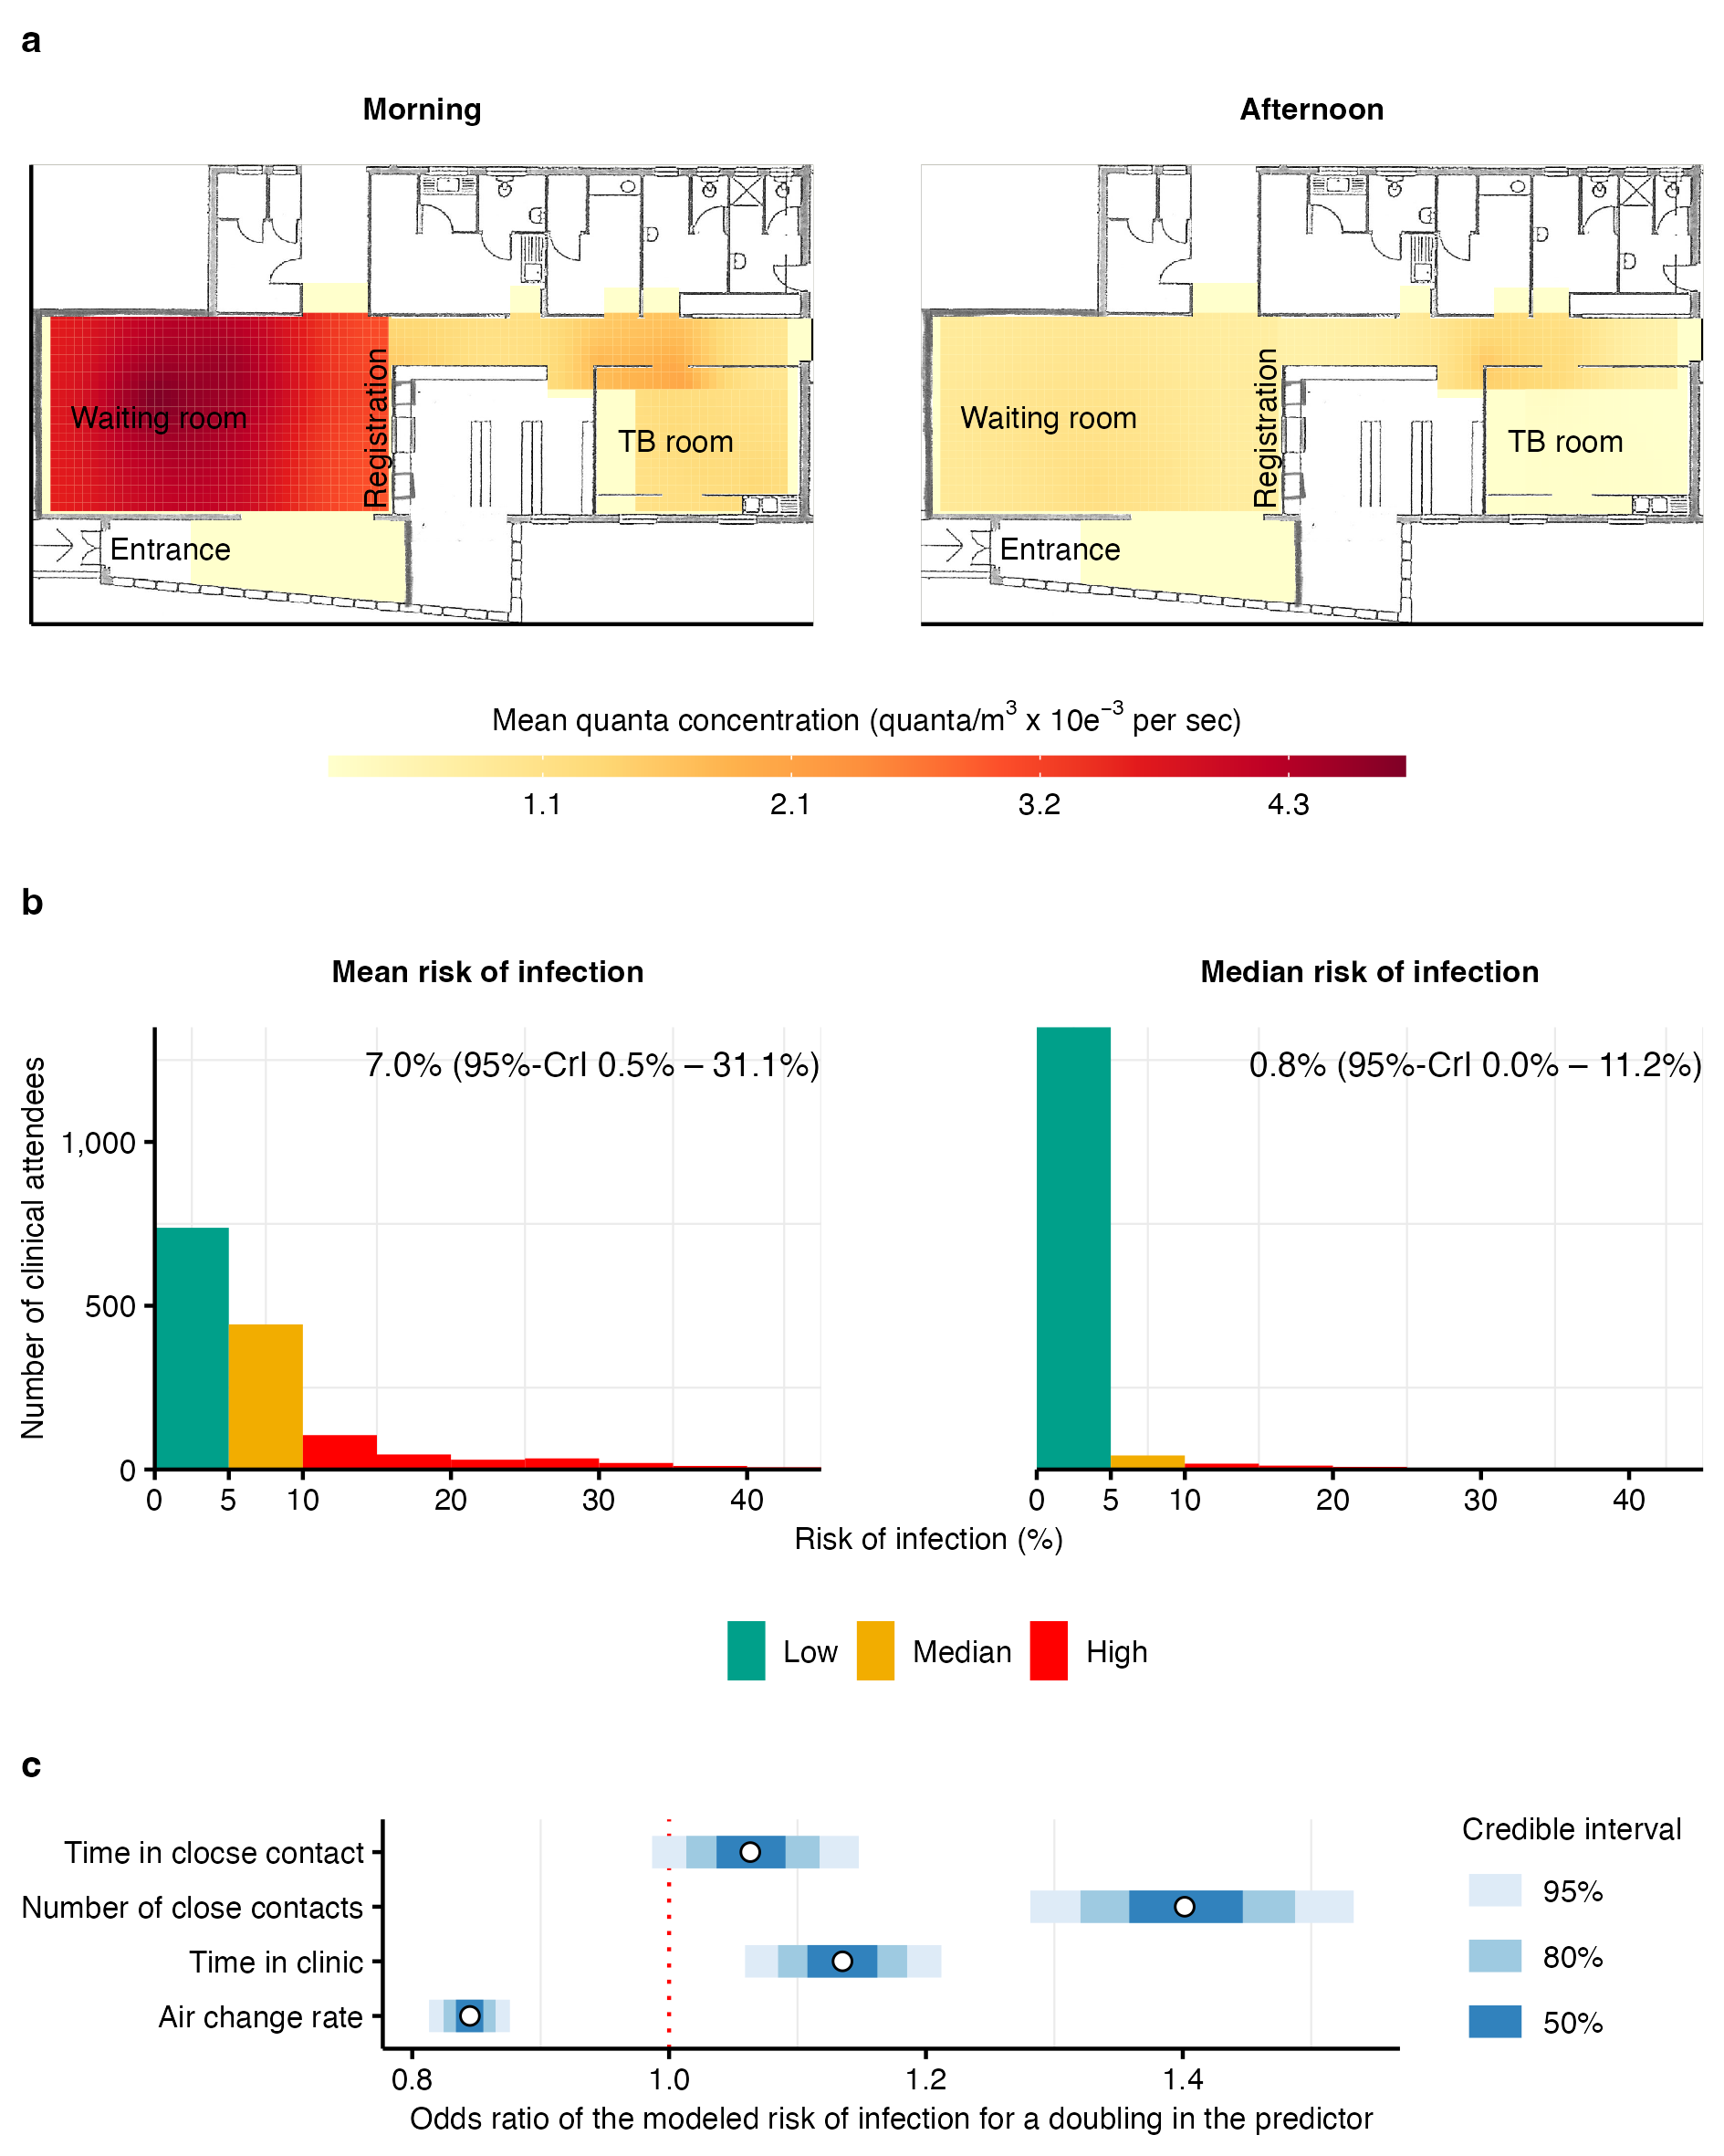
\includegraphics{results/modeling/main-figure.png}
    \caption{\textbf{Spatiotemporal modeling results.} \textbf{(a)}~Average quanta concentration in the morning and afternoon in the clinic. \textbf{(b)}~Mean and median risk of infection per clinical attendee. Low: <5\%, Medium: 5-10\%, High: >10\%. \textbf{(c)}~Association of mean infection risk with patient movement characteristics and environmental conditions. }
    \label{fig:main-modeling-results}
\end{figure}

To assess the impact of infection control measures during the COVID-19 pandemic, we performed two hypothetical scenarios shown in the top panel of \Cref{fig:scenario-results}. If none of the attendees or staff had worn masks, the attendee-average mean risk of infection would have been almost a percentage point higher (7.8\%, 95\%-CrI 0.4\%$-$41.3\%). If the ventilation rate had been fixed at 16 air changes per hour (the average in 2019 before the pandemic), the attendee-average mean risk of infection would have been more than percentage point higher (8.4\%-CrI 0.6\%$-$41.4\%). In both scenarios, the upper credible interval is roughly ten percentage points higher, indicating that mask wearing and better ventilation considerably impact the tail of the distribution, \ie high risks of infection. To assess the impact of modeling assumptions regarding the number of infectious people in space, we performed two hypothetical scenarios shown in the bottom panel of \Cref{fig:scenario-results}. Assuming there were no undiagnosed TB patients but all attendees suspected of TB were infectious, the attendee-average mean risk of infection would have been considerably higher (13.9\%, 95\%-CrI 0.0\%$-$45.2\%). Assuming there were only undiagnosed TB patients in proportion to the prevalence of TB in the South African population, the attendee-average risk of infection would have been lower (6.3\%, 95\%-CrI 0.8\%$-$16.3\%).  

\begin{figure}
    \centering
    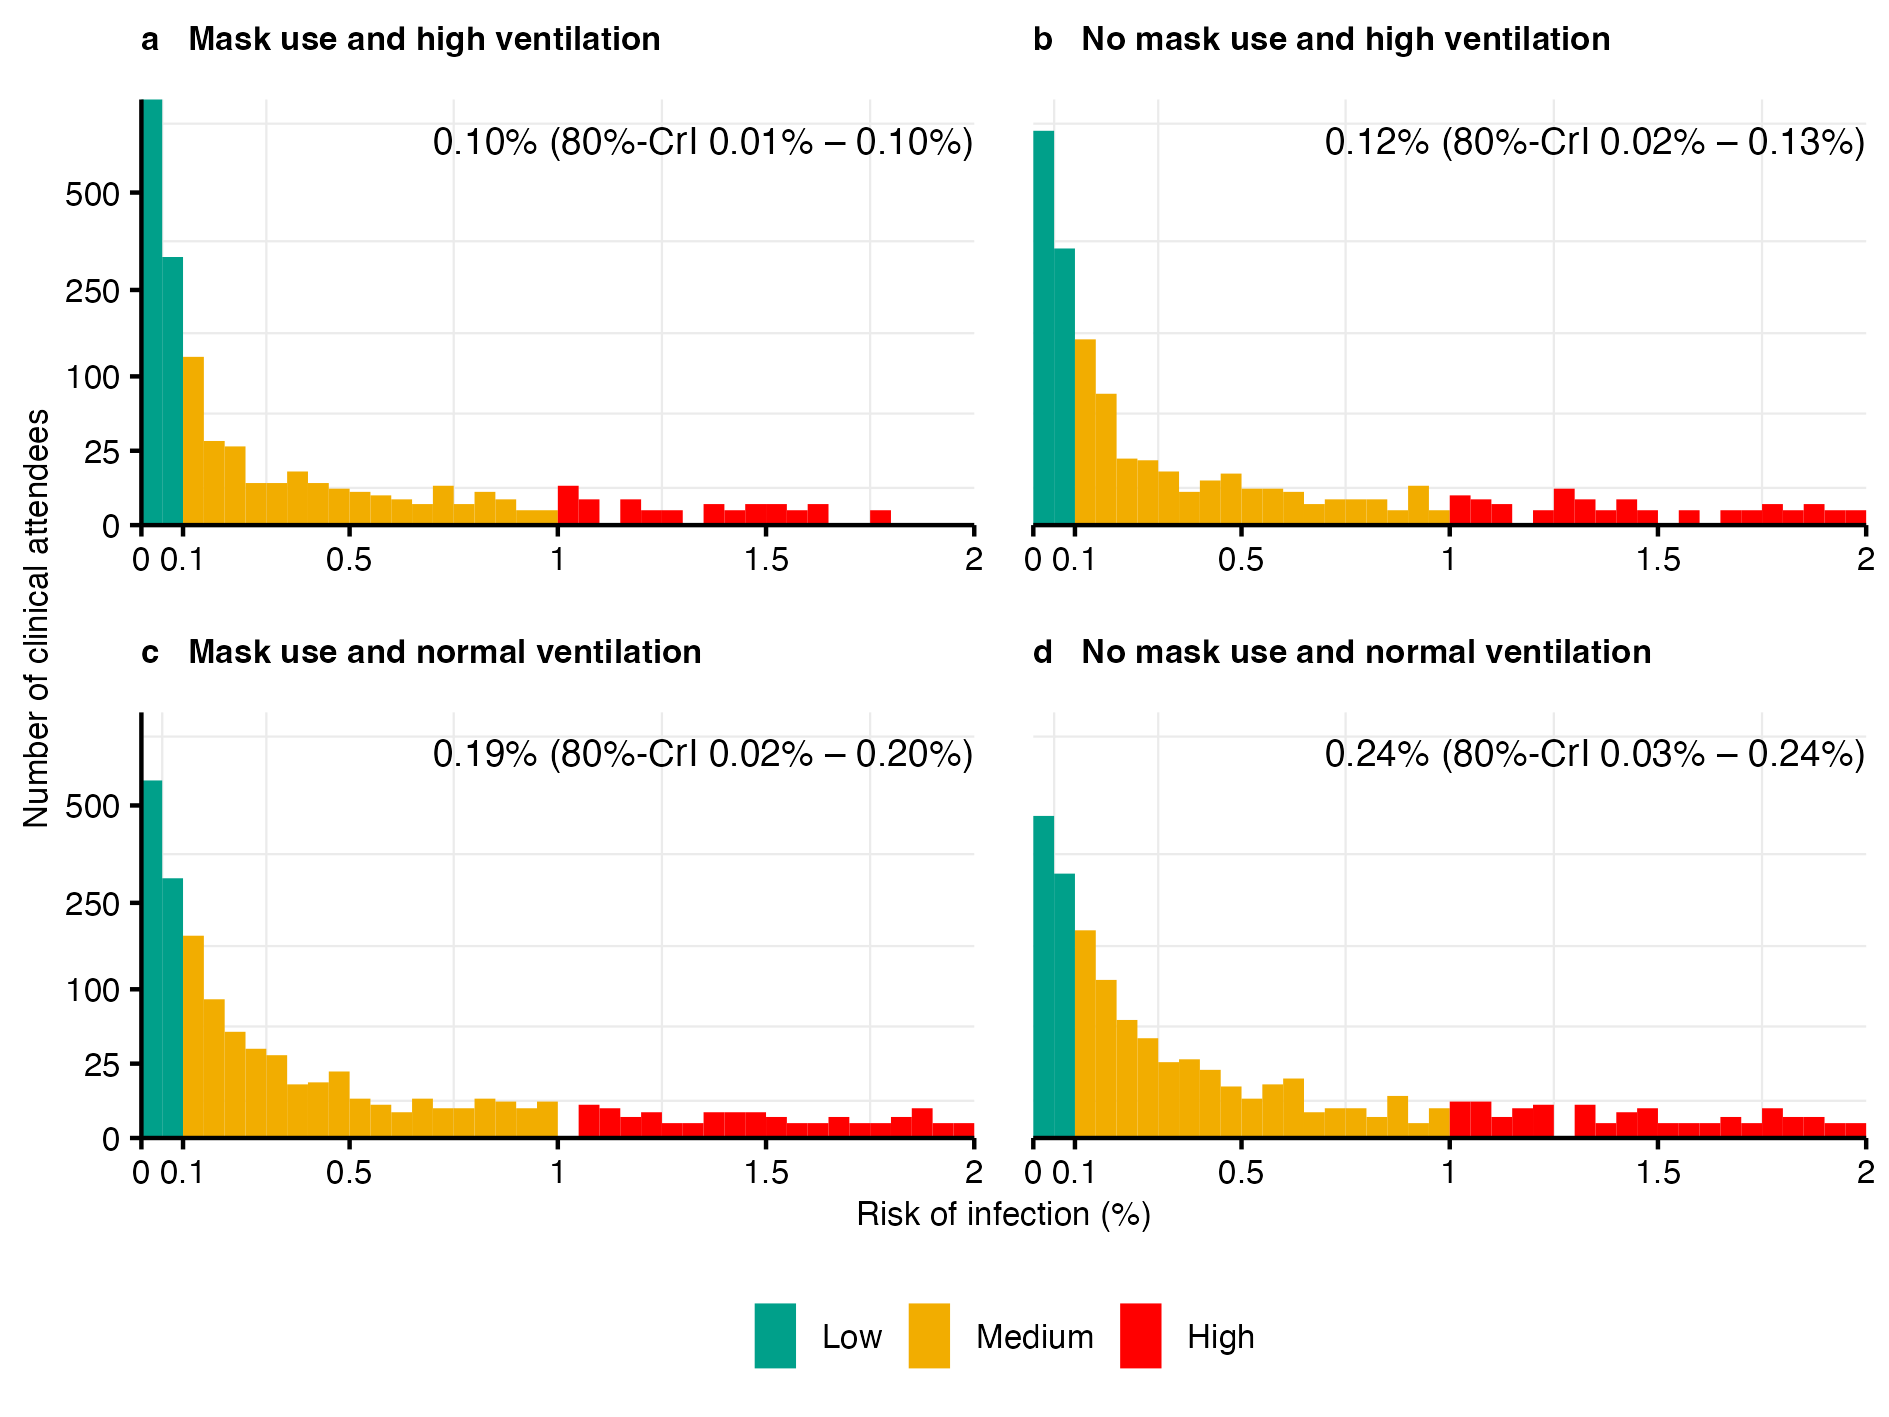
\includegraphics{results/modeling/mean-roi-comparison.png}
    \caption{\textbf{Scenario modeling results.} Mean risk of infection per clinical attendee if \textbf{(a)}~masks had not been worn by all clinical attendees and staff, \textbf{(b)}~the ventilation rate had been lower as in the year before the COVID-19 pandemic, \textbf{(c)}~the number of infectious people in the clinic corresponded to the prevalence of TB in the population, or \textbf{(d)}~the number of infectious people in the clinic corresponded to the number of diagnosed TB patients and those suspected of TB due to respiratory symptoms when attending the clinic. Low: <5\%, Medium: 5-10\%, High: >10\%.}
    \label{fig:scenario-results}
\end{figure}


\FloatBarrier

\newpage

\section{Discussion}

% summary
We developed a spatiotemporal model to estimate the concentration of infectious quanta in an indoor space and applied it to patient movement data from a South African primary care clinic in 2021 to simulate the risk of TB infection for clinical attendees. We estimated a mean risk of infection of 7\% (95\%-CrI 0.5\%$-$31.1\%) across clinical attendees. Clinical attendees with more close-contact encounters had a higher risk of infection. The modeled risk of infection would have been higher without the implementation infection control measures during the COVID-19 pandemic such as compulsory face mask wearing and better natural ventilation. 

% critical appraisal of our results
South Africa has a high burden of TB\cite{WHO2022TBReport}. A previous modeling study estimated that between 4\% and 14\% of TB transmission in adults in a high TB burden, high HIV prevalence community in South Africa occurred in primary care clinics\cite{McCreesh2022BMJGlobalHealth}. In line with this, we estimated an average infection risk of between 1\% and 16\% when assuming the number of infectious attendees is proportional to the prevalence of TB in the South African population. Another modeling study further suggests a considerable benefit of infection control measures, \eg the rate of TB transmission in clinics could be reduced by about 50\% with compulsory mask wearing and natural ventilation through opening doors and windows\cite{McCreesh2021BMJGlobalHealth}. Our modeling results also suggest a notable reduction in the average risk of infection of more than a percentage point. Moreover, we estimated a considerable shift in the tail of the risk distribution as infection control measures significantly reduce high infection risks.  

% close contacts
Our spatiotemporal model can be viewed as a modified version of the Wells-Riley transmission model\cite{Riley1978AJE}, which assumes a well-mixed airspace. By contrast, our model allows the quanta concentration to vary both over time and space. The exposure to infectious quanta therefore depends on the proximity to infectious individuals because the density of infectious particles is initially higher near them\cite{Wang2021Science,Vuorinen2020SafSci,Chen2020BuildEnv}. Our modeled risk of TB infection was significantly associated with the number of close-contact encounters and the time spent in the clinic. This result is intuitive because there are only few infectious TB patients visiting the clinic, so that more time in the clinic as well as a higher number of close contacts makes exposure to high doses of infectious particles more likely. Previous findings already suggest that prolonged close contact may be required for transmission of respiratory infections\cite{Leung2020NatMed,Brankston2007LancetID,Narasimhan2013PulmonaryMed}. However, proving close contact respiratory transmission is difficult and  empirical studies investigating the potential link between contact data and respiratory transmission are scant\cite{Voirin2015ICHE,Vanhems2013PONE}.

% more complex models and our relation
We applied our model to TB, although it can easily be extended to model other respiratory infections. Airborne respiratory transmission depends on common environmental and patient-specific factors, mainly ventilation and patient movements. Other factors such as variation in infectiousness and susceptibility, temperature and humidity, or physiochemical properties of the infectious particles can also influence the generation, diffusion, and removal of infectious quanta in the space\cite{Wang2021Science}. We discuss these factors in more depth in \supp Text~\zref{sec:depth-discussion} in \supp~Text~\zref{sec:depth-discussion}. One important factor not considered by our model is airflow, although it has been shown that poor ventilation settings can produce airflows where infectious particles are trapped in the indoor space rather than being removed\cite{Li2021BuildEnv}. Computational fluid dynamics (CFD) models can consider airflow when simulating the spatial spread of infectious particles\cite{Vuorinen2020SafSci,Jung2021InfectChemo,Li2021BuildEnv,Yan2023BE,Qian2009BE,Li2022SOTTE}. However, CFD models are computationally expensive and primarily used in experimental settings and static environments, which makes their application to our dynamic setting with patient movements difficult. Moreover, our approach requires a large number of Monte Carlo simulations to reflect uncertainty in modeling parameters and assumptions, necessitating computational efficiency. 

% limitations
Our modeling study has several limitations. Tracking patient movements with video sensors is challenging and required considerable data processing. Despite that, many patient movements were interrupted and could not be linked back together. Several important assumptions had to be made regarding the generation, diffusion, and removal of infectious quanta. Uncertainty in these modeling parameters was often large and could be reduced. For example, incorporating additional patient characteristics from the clinical database could indicate variation in infectiousness and susceptibility of patients visiting the clinic. It was not possible to validate our modeling results by empirical findings, which could be the subject of a long-term future study testing the practical implementation of our model.


% conclusions
In conclusion, our modeling study using clinical, environment, and patient movement data showed that the risk of TB transmission in a primary care clinic in South Africa in October/November 2021 was considerable, albeit mitigated by infection control measures that were implemented during the COVID-19 pandemic. The number of close-contact encounters by clinical attendees was significantly associated with their modeled risk of infection. Our spatiotemporal model could thus be used to assess the potential effectiveness of interventions targeting a reduction in the number of close contacts. 


\newpage


%TC:ignore
\section*{Acknowledgements}
...

\bibliography{references.bib}
%TC:endignore

\end{document}
